\documentclass[10pt]{article}

\usepackage{lipsum}
\usepackage{graphicx}
\usepackage{amsmath}
\usepackage{hyperref}

\usepackage{etoolbox}
\usepackage[onehalfspacing]{setspace}
\AtBeginEnvironment{figure}{\singlespacing}
\AtBeginEnvironment{table}{\singlespacing}

\usepackage{caption}
\DeclareCaptionFont{8pt}{\fontsize{8pt}{9pt}\selectfont}
\captionsetup{font={8pt}}


\usepackage[
	backend=biber,
    style=authoryear,
	url=false,
    %sorting=ynt,
    bibwarn=true,
    bibencoding=utf8,
    sortlocale=de_DE,
    maxbibnames=99,
    maxcitenames=1]{biblatex}
\renewbibmacro{in:}{}
    
\DefineBibliographyStrings{english}{
   andothers = {{et\,al\adddot}},}
   
\addbibresource{../../../bib/thesis.bib}

\AtBeginEnvironment{figure}{\singlespacing}
\AtBeginEnvironment{table}{\singlespacing}


\begin{document}


\begin{titlepage}
	\centering
	{\scshape\LARGE Ludwig-Maximilians-Universität München \par}
	{\scshape\large Faculty of Biology, Computational Neuroscience \par}
	\vspace{0.5cm}
	\includegraphics[width=0.7\textwidth]{../logo/GSN-Logo_ab35mmBreite_RGB.jpg}\par
	\includegraphics[width=0.4\textwidth]{../logo/siegel_black.pdf}\par
	\vspace{0.7cm}
	{\scshape\LARGE Report \par}
	\vspace{0.05cm}
	\vspace{0.05cm}
	{\huge\bfseries Computational Simulation of Time Perception: Model Description and Implementation \par}
	\vspace{1.5cm}
	{\Large Katharina \textsc{M Bracher} \par}
	%{Student ID: 11754625 \par}
	\vspace{0.4cm}
	{\large Supervision: Dr. Kay \textsc{Thurley} \par}
\end{titlepage}


\normalsize
\tableofcontents
%\the\textwidth 
%\makeatletter\f@size
% 345 pt = 4.79167 in -> figures 4.75 in 
% text 10 pt, fig caption 8 pt
% in drawio 10 pt -> 13.3; 8 pt -> 10.66 
\pagebreak


\section{Behavioral Effects in Magnitude Estimation}
Magnitude estimation is subject to noise that arises from external sources i.e. the statistics of the environment and internal sources i.e. neural representation of the input and the behavior.
Across sensory modalities, characteristic behavioral effects are identified (\cite{Petzschner2015}).
The most prominent observation is a regression to the mean of the stimulus range,  i.e. small stimuli are overestimated whereas large stimuli are underestimated (\textit{regression effect}). 
This effect intensifies for ranges with larger stimuli (\textit{range effect}).
For larger stimuli the standard deviation of estimates increases monotonically (\textit{scalar variability}). 
Finally, the recent history of stimuli presentations influences the current stimuli estimation (\textit{sequential effects}).
All effects mentioned above are displayed in Fig. \ref{fig:behavioraleffects}. 

Modality-independence of these effects suggests the existence of a common underlying principle or processing mechanisms, that would explain e.g. an optimal strategy for unreliable judgments due to noise (in stimuli and estimates).

\begin{figure}[ht]
	\centering
	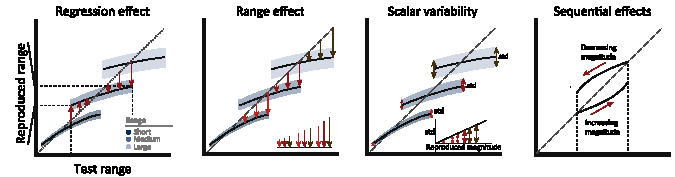
\includegraphics[width=\textwidth]{figures/behavioural_effects_petzschner.pdf}
	\caption{\textbf{Behavioral Effects} 
	\textit{Regression effect}: in a range of stimuli large stimuli are underestimated, and small stimuli are overestimated which results in a regression to the mean of the range.
	\textit{Range effect}: the regression to the mean gets more pronounced for ranges that comprise larger stimuli. 
	\textit{Scalar variability}: the standard deviation of the reproduced magnitude grows linearly with larger rages. 
	\textit{Sequential effects}: the history presented stimuli (e.g. ascending or descending order) has an influence on the reproduced magnitude. 
	Adapted from \cite{Petzschner2015}.}
	\label{fig:behavioraleffects}
\end{figure}

During time perception and time reproduction experiments, neural activity displays characteristic trajectories in a low-dimensional space ( \cite{Wang2018}, \cite{Henke2021}, \cite{Meirhaeghe2021}). 
The neural trajectories are consistently influenced by prior beliefs. 
Flexible motor timing can be achieved by controlling the speed of neural dynamics (\cite{Sohn2019}, \cite{Wang2018}). 
Further, it has been found that neural activity in anticipation of a delayed response reaches a fixed threshold with a rate inversely proportional to delay period (\cite{Murakami2014}, \cite{Mita2009}).
\cite{Wang2018} proposed a potential neural mechanism for speed control. Based on that mechanism \cite{Egger2020} developed an extended circuit model for sensorimotor timing.

\section{Model Description}
\subsection{Basic Circuit}
Flexible speed control can be achieved by a simple model consisting of three units, $u, v, y$ that represent population activity. 
The dynamics of $u, v$, and $y$ are defined as follows:
\begin{equation} \label{circuit}
	\begin{split}
	\tau\frac{\text{d}u}{\text{d}t} & = -u + \theta(W_{uI}I - W_{uv}v + \eta_u) \;, \\
	\tau\frac{\text{d}v}{\text{d}t} & = -v + \theta(W_{vI}I - W_{vu}v + \eta_v) \;, \\
	\tau\frac{\text{d}y}{\text{d}t} & = -y + W_{yu}u - W_{yv}v + \eta_y \;.
	\end{split}
\end{equation}
Two units, $u$ and $v$, receive a tonic symmetric input $I$ ($W_{uI}=W_{vI}=6$) and are mutually inhibiting each other ($W_{uv}=W_{vu}=6$). 
The inputs to $u$ and $v$ are governed by a sigmoidal activation function $\theta(x) = \frac{1}{1+exp(-x)}$.
The output unit $y$ receives excitatory input from $u$ and inhibitory input from $v$ ($W_{yu}=W_{yv}=1$) which results in a ramp-like activity of $y$.
All three units have a time constant $\tau = 100$ ms. 
Stochastic synaptic inputs are modeled as independent white noise $\eta_u, \eta_v, \eta_y$ with standard deviation $\sigma$.
Initial conditions of $u, v$ and $y$ have been optimized for in \cite{Egger2020} and are set to $u_0=0.7 , v_0=0.2 , y_0=0.5$ (Fig. \ref{fig:circuit}a)

Depending on the input $I$, the system shows different dynamics. For low levels of $I$ (0$<$I$<$0.5) the system has three fixed points (two stable, one unstable at $u=v$) and $y$ ramps up faster the higher input $I$. 
For intermediate values of $I$ (0.5$<$I$<$1) the system still shows three fixed points of the same sort as in the low input regime (Fig. \ref{fig:circuit}b)but $y$ ramps up with a slope that is inversely proportional to the input $I$ ($y$ ramps up slower the higher input $I$, see Fig. \ref{fig:circuit}c). 
For high $I$ (1$<$I) the system has one stable fixed point (at $u=v$) and $y$ ramps down faster for higher $I$.
Thus, the speed at which the output $y$ evolves can be controlled by the input $I$ (Fig. \ref{fig:circuit}d) and determines the time interval after which $y$ reaches a fixed threshold $y_{\text{th}}$. 
In interval reproduction experiments, reaching a threshold $y_{\text{th}}$ can be understood as movement initiation time which can be controlled for by adjusting $I$.
In this report, the intermediate input regime is explored: higher inputs result in a shallower slope of $y$, such that the threshold $y_{\text{th}}$ is reached after a longer time interval.

%%%%%%%%%%%%%%%%%%%%%%%%%%%%%%%%%%%%%%%%%%%%%%%%%%%%%%%%%%%%%%%%%%%% nullclines
\begin{figure}[ht]
	\centering
	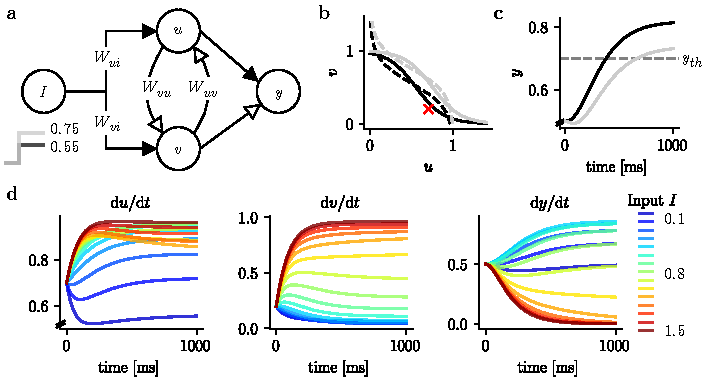
\includegraphics{figures/defCircuit_nullcl.pdf}
	\caption{\textbf{Basic Circuit and Input Regimes} 
	\textbf{(a)} $u$ and $v$ share a common input $I$. The input is governed by weights $W_{uI}$ and $W_{vI}$. The two units have reciprocal inhibitory connections with weights $W_{uv}$ and $W_{vu}$ that determine the inhibitory strength. Both project to the output unit $y$ with an excitatory connection from $u$ and an inhibitory connection from $v$. Excitatory and inhibitory connections are shown by filled and open arrows, respectively. 
	\textbf{(b)} The control of the speed in $y$ can be analyzed in the phase plane of $u$ and $v$. The $u$ (dashed) and $v$ nullcline (solid) is shifted when the input is increased from $I=0.65$ (black) to $I=0.75$ (gray). In the intermediate regime the systems shows two stable and one unstable fixed point. The red cross indicated the initial conditions for the dynamics in (c). Depending on $I$, with the same initial conditions, the system evolves faster or slower to the stable fixed point. 
	\textbf{(c)} Dynamics of $y$ for intermediate regime with input $I=0.75$ in gray and $I=0.65$ black. There is an inverse relation of input strength and slope. With higher input, the threshold at 0.7 (dashed line) is reached after a longer time interval. 
	\textbf{(d)} Dynamics of $u, v, y$ for inputs from $0.1\leq I \leq 1.5$ are shown. Initial conditions are set to $u_0=0.7 , v_0=0.2 , y_0=0.5$. With these initial conditions and values of $I>=0.5$, the relation of steady state activity of $y$ (and slope to reach the steady state) is inverse to $I$ (intermediate and high $I$ regime). For values $I<=1$ the activity of $y$ ramps down (yellow corresponds to $I=1$). For $I<0.5$ the steady state (slope) is smaller the smaller $I$ (low $I$ regime, dark blue).}
\label{fig:circuit}
\end{figure}

\subsection{Update Mechanism and Experiment Procedure}
Basic interval reproduction experiments can be designed with only two epochs: a measurement epoch that has the duration of the stimulus interval and a reproduction epoch that starts immediately after the measurement epoch (Fig. \ref{fig:epochs}b). 
The basic circuit described above is modified to perform interval reproduction (see Figure \ref{fig:epochs}a for schematic of modified circuit).
The relation of input $I$ with the slope of the ramping activity of $y$ is used in combination with a fixed threshold $y_{\text{th}}$.
By adding an update mechanism that flexibly adjusts $I$, the threshold crossing of $y$ can be delayed or moved to earlier times.
This way, measuring and reproducing an interval is done predictively, by adjusting the slope of the ramp such that the output reaches the threshold after the intended time.
%In other scenarios, time could be encoded by the level a ramp reaches with a fixed slope.
In the model the measurement epoch is fixed to the stimulus interval $t_s$, and the reproduction epoch ends, when $y$ reaches the fixed threshold $y_{\text{th}}$ from below. 
The time from the end of the measurement epoch until the threshold-crossing of $y$ yields the reproduced time interval $t_r$ that is aimed to equal the stimulus interval $t_s$ (Fig. \ref{fig:epochs}c).

\begin{figure}
	\centering
	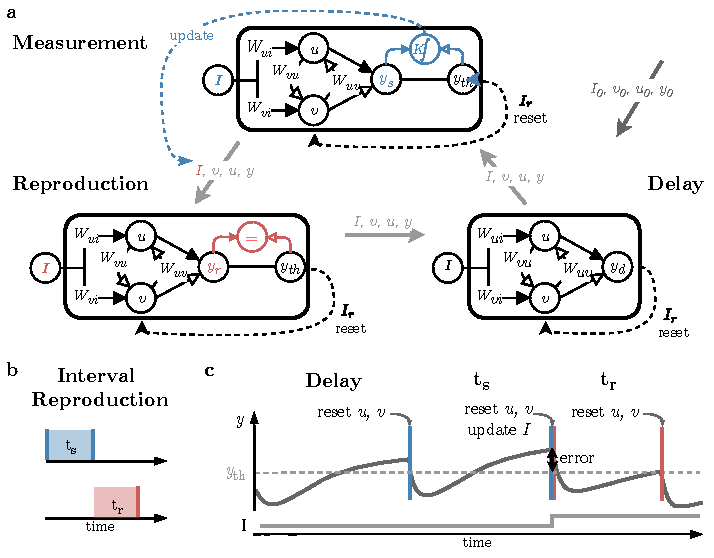
\includegraphics{figures/epochs.pdf}
	\caption{\textbf{Extended Circuit for Experiment Simulation} 
	\textbf{(a)} The circuits for measurement, reproduction and delay epoch are displayed. All circuits comprise the same basic structure with different additional elements that are unique for the epoch. Initial values of $u, v, y$ and $I$ are fed into the delay circuit for the duration of the initial interval. $u$ and $v$ are reset with a transient input $I_r$ before end values of $u, v, y$ and $I$ are transferred to the measurement circuit as new initial conditions. After the duration of the stimulus interval the difference between $y$ and the threshold $y_{\text{th}}$ is used with the memory parameter $K$ to update $I$ together with another reset of $u$ and $v$. The values are transferred with all other variables to the reproduction circuit. The reproduction epoch ends when $y$ reaches the threshold $y_{\text{th}}$ from below. Before the presentation of another stimulus interval, there is again a delay period with no update of $I$. The reset mechanism enables the model to simulate an arbitrary number of stimulus intervals. Adapted from \cite{Egger2020}.
	\textbf{(b)} Interval reproduction experiment with stimulus interval $t_s$ (blue) and reproduction $t_r$ (red).
	\textbf{(c)} Schematic of one trial. After a delay epoch $u$ and $v$ are reset. The measurement epoch lasts for the duration of the stimulus interval $t_s$. $y$ should reach the threshold $y_{\text{th}}$ (dashed line) at exactly the time the stimulus interval ends. The threshold was crossed well before the end of the interval and at the end of the measurement epoch, the error in $y_m$ to the threshold $y_{\text{th}}$ is used to update $I$. To reach the threshold at a later time, $I$ is increased, which reduces the slope of $y$ in the reproduction epoch. After the reset of $u$ and $y$ and the update of $I$ the reproduction ends when $y$ reaches the threshold. The time after the reset and update until the threshold crossing denotes the reproduced interval $t_r$.}
\label{fig:epochs}
\end{figure}

The following update mechanism of $I$ is based on the intermediate input regime, that shows an inverse relation of $I$ to the slope of $y$ (Fig. \ref{fig:circuit}b).
The error signal is determined at the end of the measurement epoch and is composed of the difference of $y$ to the threshold $y_{\text{th}}$.
If the threshold $y_{\text{th}}$ is not reached during the measurement epoch, the slope has to be adjusted, such that y ramps up faster to reach the threshold at exactly the time of the stimulus interval. For a steeper slope, $I$ is reduced.
If $y$ crossed the threshold before the measurement epoch ends, so is above $y_{\text{th}}$ by the end of the stimulus interval, the slope needs to be reduced in order to reach the threshold at a later time in the reproduction. For a shallower slope, $I$ is increased (Fig. \ref{fig:epochs}c).
$I$ is adjusted according to the error $(y-y_{\text{th}})$, weighted by a memory parameter $K$ right at the end of the measurement epoch
\begin{equation} \label{Iupdate}
	\begin{split}
	\tau\frac{\text{d}I}{\text{d}t} & = sK(y-y_{\text{th}}) \;.
	\end{split}
\end{equation}
The update of $I$ is only active for a pulse between the measurement and reproduction epoch ($s=1$) and inactive for all other times ($s=0$).
Further, $u$ and $v$ receive a transient input pulse $I_r$ to reset the dynamics for the subsequent epoch (Fig. \ref{fig:epochs}c)
\begin{equation} \label{experimentcircuit}
	\begin{split}
	\tau\frac{\text{d}u}{\text{d}t} & = -u + \theta(W_{uI}I - W_{uv}v + \eta_u - I_r) \;,\\
	\tau\frac{\text{d}v}{\text{d}t} & = -v + \theta(W_{vI}I - W_{vu}v + \eta_v + I_r) \;.\\
	\end{split}
\end{equation}
Resetting the dynamics after the reproduction epoch enables the model to simulate an arbitrary number of stimulus intervals. 
Before a new stimulus presentation there is a delay period: In the beginning of an experiment with a sequence of stimuli there is an initial interval with the initial values of $u, v, y$ and an initial input $I_0$ (Fig. \ref{fig:epochs}c). 
This additional interval in the beginning of the experiment allows the model to get closer to steady-state before the stimulus presentation starts. 
Reproductions that do not reach the threshold in a certain time span  or too early are classified as timeout trial.
%sup

To simulate variability in the reproductions as it is found in real data, noise is added to $u, v$ and $y$ in the implementation. In data an monotonic increase of the standard deviation of reproductions is found (\textit{scalar variability}). 
If noise levels in the model are too high ($\sigma>0.2$) the standard deviation of reproductions is not growing monotonically with $\sigma$ (\cite{Egger2020}).
For all simulations $\sigma$ was set to 0.02 (Supplementary Fig. \ref{sup:rangeCV}b, c).
For an example experiment with a sequence of five trials see Figure \ref{fig:experiment}a. 
In the full simulation 500 stimuli, randomly chosen from a stimulus range, were presented. 
The stimulus range consisted of seven uniformly distributed stimuli from short and long stimulus range 400-700 ms for the short range and 700-1000 ms for long range. The ranges both contained a 700 ms stimulus interval (Supplementary Fig. \ref{sup:rangeCV}a).
This results in a distribution of reproduced time intervals for each stimulus and a distribution of inputs that drive the reproduction (Fig. \ref{fig:experiment}b).
Taking the mean over the distribution of reproduction times for each stimulus allows for the investigation of effects in the behavioral results (Fig. \ref{fig:parameter}c). 

\begin{figure}[ht]
	\centering
	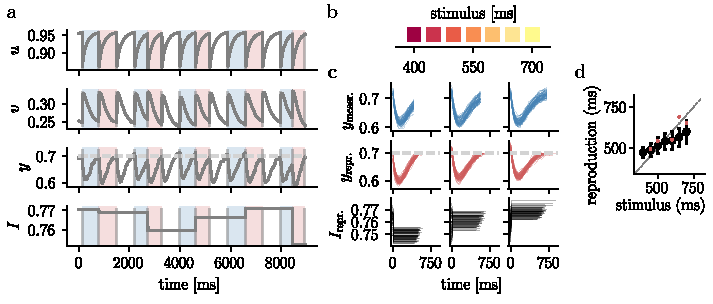
\includegraphics{figures/trial.pdf}
	\caption{\textbf{Experiment Simulation} 
	\textbf{(a)} Example trial with a sequence of five stimulus intervals (600, 600, 500, 700, 600, 400 ms). Initial values are set to $u_0=0.7 , v_0=0.2 , y_0=0.5. I_0=0.8$, other parameters are $\sigma=0.01$, the initial duration of 750 ms and a 700 ms delay period before new stimuli. The dynamics of $u, v, y $ and $I$ are displayed over time. The threshold is set to $y_{\text{th}}=0.7$ (dashed line). The first stimulus interval is reproduced poorly as the system needs more trials to adapt the initial $I_0$ to a suitable range (reproduced times 1140, 820, 690, 660, 650, 570 ms).
	\textbf{(b)} The measurement (upper) and reproduction (middle) epoch and input for reproduction (lower) are shown over the course of the full experiment with the short stimulus range. The experiment consisted of 500 trials with randomly chosen stimuli from a stimulus range consisting of seven stimuli from 400 to 700 ms. All trials are sorted according to the stimulus and displayed together. Shown are trials for stimuli of 400, 550 and 700 ms.}
\label{fig:experiment}
\end{figure}

%%%%%%%%%%%%%%%%%%%%%%%%%%%%%%%%%%%%%%%%%%%%%%%%%%%%%%%%%%%%%%%%%%%%%%%%%%%%%%%%%%%5
\section{Memory Parameter in Accordance with Error Minimization}
\subsection{Behavioral Plausible Slopes}
We asked whether the observed behavioral effects in real data (Fig. \ref{fig:behavioraleffects}) can be reproduced by experiment simulations with the circuit model. 
A crucial parameter is the memory parameter $K$, which defines the weight with which the input is adjusted to balance the mismatch between the predicted interval and the stimulus duration. 
In stable parameter regimes, the reproductions show a regression to the mean. 
Biological plausible slopes in behavioral results lie around 0.83 for the short and 0.73 for the long range (\cite{Thurley2018}, \cite{Jazayeri2010}). 
Choosing certain values for $K$, the model produced plausible slopes for various time constants (Fig. \ref{fig:parameter}a), where $K$ has to be adjusted according to the stimulus range. $K$ is set to smaller values for the long range, putting less weight on the update compared to the short range, to produce plausible slopes.

\subsection{Optimization of $K$}
Can behavioral effects also be achieved by adjusting $K$ in accordance with error minimization?
To find optimal values for $K$ the minimized the mean squared error was used, defined as the sum of the squared bias and variance of the mean reproductions (Supplementary Eq. \ref{MSE}).
For larger time constants $\tau$ the optimal $K$ increased. For all time constants optimal values of $K$ were smaller for the long range compared to the short range, as already found for values of $K$ that result in plausible slopes.
The corresponding time constant $\tau$ for the overall minimum of the MSE differed between the two stimulus ranges. For the short stimulus range, $\tau = 120 ms, K= 11$ yielded the overall minimum, for the long range the parameter pair was $\tau = 200 ms, K= 20$(Fig. \ref{fig:parameter}b, Supplementary Fig. \ref{sup:othererror}a, b). 
For the experiment simulation we chose a common $\tau$ for the short and long range of 140 ms. Corresponding optimal values for $K$ were 14 for the short and 10.5 for the long range. 
Behavioral results show a regression to the mean with a stronger regression for the long range (range effect) (Fig. \ref{fig:parameter}c). For dynamics of $y$ over the whole experiment see Supplementary Fig. \ref{sup:experiment}).
Adjusting $K$ in accordance with error minimization, leads to putting more weight on the prior experience for longer stimuli, which naturally entail more uncertainty, and is thus biological plausible.
Yet, the slope for the small ranges lies below the slopes found in data. 
The standard variation of reproductions increases linearly (scalar variability), the mean coefficient of variation (CV) for the short range is 0.09, for the long range 0.11 (Fig. \ref{fig:parameter}d).
Furthermore, a general underestimation for the large range is observed for all time constants (Supplementary Fig. \ref{sup:othererror}e). This is probably the case due to high variance that pushes $K$ to lower values.
When optimizing for the squared bias or variance only, no range effect is observed and the relation of smaller $K$ for longer stimuli, so putting more weight on the prior is not apparent for both options (Supplementary Fig. \ref{sup:othererror}c, d).  
%supp

\begin{figure}[ht]
	\centering
	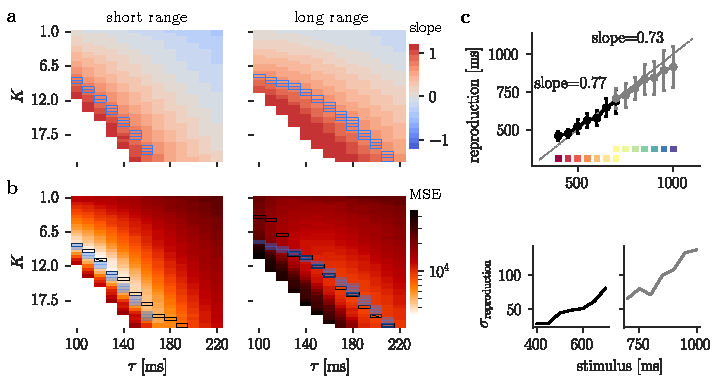
\includegraphics{figures/interIparams.pdf}
	\caption{\textbf{Behavioral Effects and Parameter Optimization} 
	\textbf{(a)} Simulations with 500 trials for each pair of memory parameter $K$, and time constant $\tau$ at noise level $\sigma = 0.02$. Simulations were performed with stimuli chosen from the short (left) or long range (right). Color scale represents the slope for each experiment stimulation, which describes the behavioral results. A slope of 1 on the identity line corresponds to perfect reproduction of the stimuli. Behavioral plausible slopes are encircled. Empty spaces show simulations, that exceeded the number of timeout trials and where thus excluded from analysis.
	\textbf{(b)} Optimization of the weight given to the update, $K$, for different time constants $\tau$ at noise level $\sigma = 0.02$. Color scale represents the MSE for an experiment stimulation with 500 trials for each pair of $K$ and $\tau$. Stimuli were either chosen from the short (left) or the long stimuli range. The minimal error for each $\tau$ is encircled in black. The minimal error across all $\tau$ is encircled in blue. 
	\textbf{(c)} Mean reproductions for simulation with 500 trials for each stimulation with the short (black) and long (grey) stimulus range. The value of $K$ is optimized for a time constant of $\tau = 140 ms$. For the simulation with short stimulus range optimal $K$ was 14, with the long stimulus range optimal $K$ was 10.5. If the mean lies on the identity line, reproductions corresponds to the stimulus time interval.  
	\textbf{(d)} Standard deviation of reproductions for each stimulus for the short ad long range from the simulation in (c).
	}
\label{fig:parameter}
\end{figure}
%%%%%%%%%%%%%%%%%%%%%%%%%%%%%%%%%%%%%%%%%%%%%%%%%%%%%


\pagebreak
\setcounter{section}{0}
\addcontentsline{toc}{section}{Supplements}
\section*{Supplements}
\setcounter{figure}{0}
\setcounter{table}{0}
\setcounter{equation}{0} 
\renewcommand{\figurename}{Supplementary Figure}
\renewcommand{\tablename}{Supplementary Table}

\section{Methods}
\subsection*{Circuit}
For simulating the dynamics of $u, v, y$ and $I$ Euler's method was used with a step size $\Delta t$ set to 10 ms.
The reset mechanism of $u$ and $v$ is switched on for one time step after every epoch and the update mechanism of $I$ is switched on for one time step after the measurement epoch only.
Noise is independently sampled for every time step from a Gaussian distribution with standard deviation $\sigma$.

\subsection*{Timeouts}
Reproductions that do not reach the threshold in a certain time span (twice the stimulus interval) are classified as timeout trials. 
If the threshold is crossed particularly early, the trial is also classified as (early) timeout trial (crossing before 0.2 of stimulus interval).
Simulations that exceed a fixed number of timeout trials (10\% of all trials in the experiment) were excluded from analysis. If timeout trials occurred for a single stimulus more than 10\% of all trials of this stimulus, the simulation was also discharged.
This only happened for unfavorable parameter regimes.


\subsection*{Experiment Simulation}
In all simulations in the intermediate regime, the threshold $y_\text{th}$ was set to 0.7. The model worked with higher and lower thresholds robustly.  
For experiment simulations with 500 trials, the increase of the standard deviation of reproductions plateaus with noise levels $\sigma > 0.1$. This was tested with parameters set to $\tau=100$, $K_\text{short}=8.5$ and $K_\text{long}=6$.
The standard deviation of reproductions grows monotonically for increasing stimulus intervals for tested noise levels (Supplementary Fig. \ref{sup:rangeCV}b).
Further, the coefficient of variation (CV) was used to quantify the degree of variation. It is defined as $\text{CV}=\frac{\sigma_\text{reproduction}}{\mu}$ for each stimulus, where $\mu$ corresponds to the stimulus interval and $\sigma_\text{reproduction}$ to the standard deviation of the corresponding reproductions. 
To achieve variations close to real data, reproductions should have a CV of 0.2 to 0.4 that is constant over all stimulus intervals (Supplementary Fig. \ref{sup:rangeCV}c).
For all simulations the noise level $\sigma$ was set to 0.02, where the mean CV for the short range was 0.1 and for the long range 0.15 with the parameters from above.

In all experiment simulations, a series of 500 trials was presented to the model.
Stimuli were randomly chosen from the short (400-700 ms) or the long (700-1000 ms) stimulus range (Supplementary Fig. \ref{sup:rangeCV}a).
The stimulus series had a uniform distribution of stimuli, a repetition of all seven stimuli in every 20 trial windows and no remarkable oscillation.
To allow for optimization of $K$ the same stimulus series was used. Added noise was initialized equally to extract changes in results only based on parameter changes.
Different noise initialization influence the optimal value of $K$ slightly. For 20 simulations with $\tau=140$ and $\sigma=0.02$ the mean optimal $K$ and standard deviation for the short range were $K = 14.45$, std = 0.49 and for the long range $K = 9.91$, std = 0.77. 

\begin{figure}[ht]
	\centering
	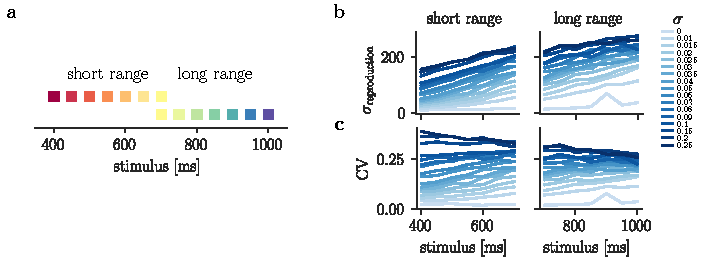
\includegraphics{figures/supp_interI.pdf}
	\caption{%\textbf{xx} 
	\textbf{(a)} For experiment simulation two stimuli ranges were used. The short range contained stimuli from 400 to 700 ms, the long range contained stimuli from 700 to 1000 ms.
	\textbf{(b)} Standard deviation of reproductions for each stimulus in an experiment simulation with 500 trials and $\tau=100$. $K$ was set to 8.5 and 6 for the short and long range respectively. 
	\textbf{(c)} Same as (b) but standard deviation of reproductions normalized by stimulus duration.
	}
\label{sup:rangeCV}
\end{figure}

\begin{figure}[ht]
	\centering
	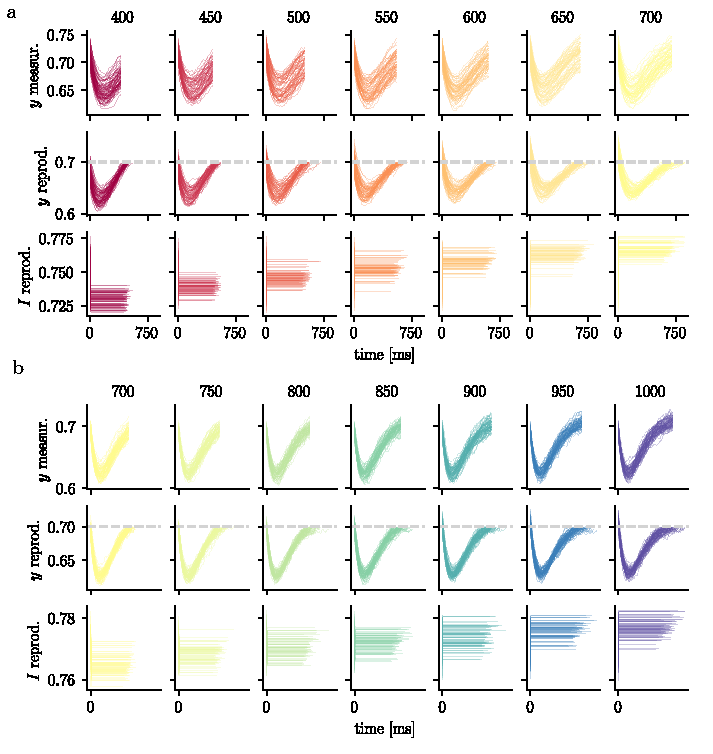
\includegraphics{figures/supp_experiment.pdf}
	\caption{\textbf{Experiment simulation with optimized $K$}
	\textbf{(a)} For an experiment simulation with 500 trials, a time constant $\tau$ of 140 and optimal $K=14$, the activity was sorted according to epoch and stimulus interval. Stimuli were chosen from the short range. Upper row show the behavior of $y$ in the measurement epoch, middle row shows the behavior of $y$ in the reproduction epoch. The lower row shows the input level to the circuit during the reproduction epoch. 
	\textbf{(b)} Same as (a) with stimuli chosen from the long range and $K$ set to 10.5. 
	}
\label{sup:experiment}
\end{figure}

\subsection*{Optimality by Minimizing MSE}
We minimized the error in the interval reproductions across the experiment, we defined the $\text{MSE} = \text{bias}^2+\text{var}$, with the bias specified as the squared difference between the mean reproduction $\bar{t_{r}}$ for each stimulus interval $t_s$ in the stimulus range $S$ and variance as mean $\sigma^2$ for all stimuli intervals in $S$.
\begin{equation} \label{MSE}
	\begin{split}
	 \text{bias} & = \frac{1}{S} \sum \limits_{i=1}^{S} (\bar{t_{r_i}} - t_{s_i}) \;,\\
	 \text{bias}^2 & = \frac{1}{S} \sum \limits_{i=1}^{S}(\bar{t_{r_i}} - t_{s_i})^2 \;,\\
	 \text{var} & = \frac{1}{S} \sum \limits_{i=1}^{S}(\sigma_i^2) \;.\\
	\end{split}
\end{equation}

%%%%%%%%%%%%%%%%%%%%%%%%%%%%%%%%%%%%%%%%%%%%%%%%%%%%%%%%%%%%%%%%%%%%%%%%%%%%%%%%%%%
\subsection*{Optimization with Other Errors}
Optimal values of $K$ are based on the MSE, which composed of the squared bias and the variance of reproductions. 
Time constants $\tau$ with the minimal MSE for a value of $K$ differ between the short and the long range. For the short range the optimal time constant $\tau = 120 ms$, for the long range $\tau = 200 ms$ (Supplementary Fig. \ref{sup:othererror}a, b). If optimization is based only on the squared bias, optimal time constants are 100 ms for the short and 110 ms for the long range. 
The variance is pushing the optimal time constant to lager values for both stimulus ranges. 
Similarly, optimal $K$ is pushed to lower values by the variance (Supplementary Fig. \ref{sup:othererror}c, d).
For all optimized values, be it on the squared bias, the variance or combined in the MSE, there is a general underestimation of stimulus intervals from the long range, which becomes appeared in Supplementary Fig. \ref{sup:othererror}e.

\begin{figure}[ht]
	\centering
	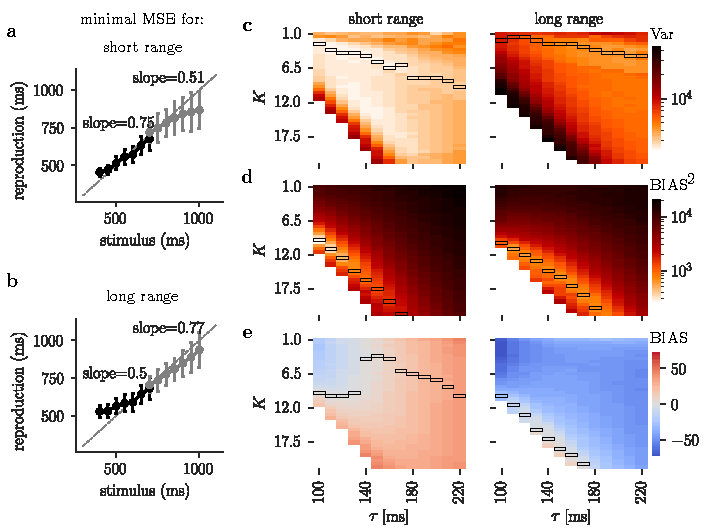
\includegraphics{figures/supp_othererror.pdf}
	\caption{%\textbf{Optimization based on Variance, BIAS\textsuperscript{2} and BIAS}
	\textbf{(a)} Behavioral results for a simulation with 500 trials, $\sigma = 0.02$ and optimized time constant $\tau$ for the short range ($\tau = 120$). For simulations with both short and long range, the optimal time constant for the short range was used. Optimal $K$ for $\tau = 120$ was 11 for the short, 7 for the long range.
	\textbf{(b)} Same as (b) with optimized $\tau$ for the long range ($\tau = 200$). Optimal $K$ for this time constant was 25 for the short range and 20 for the long range. 
	\textbf{(c)}  Simulations with 500 trials for each pair of memory parameter $K$, and $\tau$ at noise level $\sigma = 0.02$. Simulations were performed with stimuli chosen from the short (left) or long range (right). Color scale represents the variance of reproductions in the behavioral results.
	\textbf{(d)} Same as (c), color scale represents the squared bias of reproductions.
	\textbf{(e)} Same as (d), color scale represents the bias of reproductions. Values larger than 0 correspond to an overestimation, values smaller than 0 to an underestimation of the stimulus interval.
	}
\label{sup:othererror}
\end{figure}

\section{Comparison of Intermediate and High Input Regime}
% two fixed points
In the intermediate input regime higher $I$ result in a shallower slope of $y$.
% one fixed point, high activity
% relation I and slope in circuit
% reset inpulse opposite, and 10 times higher
% initial I over 1
% threshold over 0 -0.2
% higher I results in steeper slope

% Figure: phase plane comparison
% Figure: different inputs, relation I and slope, bsp behavior u, v, y, I

\begin{figure}[ht]
	\centering
	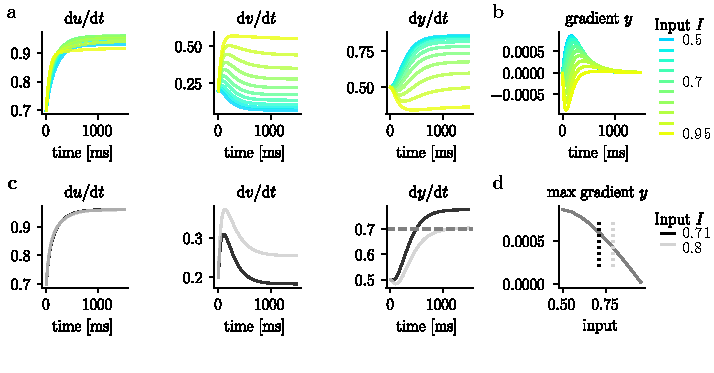
\includegraphics{figures/supp_interIregime.pdf}
	\caption{\textbf{xxx}
	\textbf{(a)}
	\textbf{(b)}
	\textbf{(c)} 
	\textbf{(d)} 
	}
\label{sup:interI}
\end{figure}

\section{Design}
The code is designed in a modular way, such that multiple types of experimental procedures with shared functionality are accessing the same basic circuit, which is implemented in \texttt{BaseSimulation} as shown in Figure \ref{fig:code}.
The implementation of the basic circuit can be reused for all epochs.
Different experiments can have different result types, all of which can be found in \texttt{result.py}. After each experiment, the results are gathered and stored together, consisting of the parameter set, the simulation time course, a list of reset time points, a list of production times, a list of indices of timeout trials and the stimulus list.
Analysis of the results is performed in the same file. Depending on the analysis (e.g. behavioral), different plots are implemented in \texttt{plot.py} to visualize the results. 

All parameters are set and described in \texttt{Params} and can be modified individually or by reading a parameter dictionary. The parameters configure the circuit. 
To initiate a simulation, the parameter set is handed to one of the implemented experiments. 
An interval reproduction experiment, as described in this report is implemented in \texttt{experiment\_simulation.py}. 
Parallel simulations of one trial (one delay, measurement and reproduction epoch) is implemented in \texttt{parallel\_simulation.py}.
Both \texttt{experiment\_simulation.py} and \texttt{parallel\_simulation.py} contain a simulate function that accesses the base simulation (\texttt{BaseSimulation}) with the implementation of the basic circuit.
For each epoch or update/reset step, the simulate function feeds the according time steps and initial conditions into the network in \texttt{BaseSimulation}. Depending on the epoch, the reset and update mechanism are tuned on or off. 
After each epoch or pulse, the results of the network are joint to the time course of the experiment in trial\_update. The simulate function returns a \texttt{SimulationResult} or \texttt{RangeParallelSimulationResult} object.

For an overview of the code structure see Figure \ref{fig:code} and for its usage see simulations.ipynb at \href{https://github.com/KatharinaBracher/MScThesis}{github.com/KatharinaBracher/MScThesis}. 

\section{Implementation}
All simulations and analysis were performed with Python 3.9.7. 
The following libraries were used: matplotlib (3.5.1), NumPy (1.22.3), SciPy (1.8.0), scikit-learn (1.0.2). 
An experiment simulation can not be parallelized, since each step depends on the previous one.
% For the parameter search multiple experiment simulations were parallelized 

% server

\begin{figure}[ht]
	\vspace*{-2cm}
	\makebox[\textwidth][c]{\includegraphics[width=1.2\textwidth]{figures/codeStructure.drawio.pdf}}
	\caption{\textbf{Design} The base simulation and different procedures (experiment, parallel) are all implemented in separate files. All results and analysis are collected in \texttt{result.py}, all plot for different result types are collected in \texttt{plot.py}}
\label{fig:code}
\end{figure}


\clearpage
\addcontentsline{toc}{section}{References}
\printbibliography




































\end{document}